\section{Användning av det grafiska gränssnittet}

Det grafiska gränssnittet finns där för att kontrollera och få information om systemets status.

\begin{figure}[h!]
	\center
	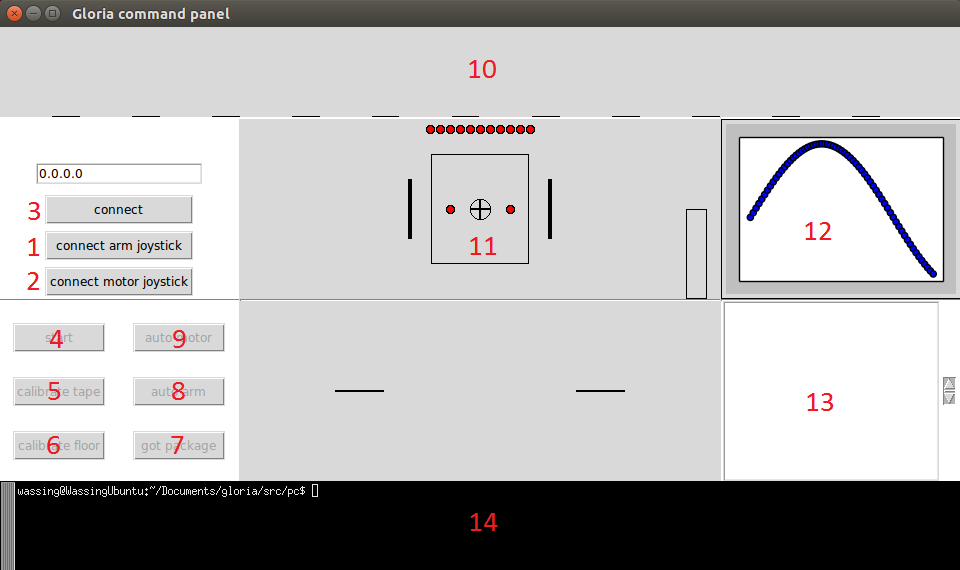
\includegraphics[scale=0.6]{Gui.png}
	\endcenter
	\caption{Gui. Överst visas information från linjesensorn (10), i mitten visas en översikt av systemet (11), till höger visas reglerfel (12) samt felmeddelanden (13), nedre mitten visar motorernas hastighet (14) och nederst visas en terminal (15).}
\end{figure}

\subsection{Initiering och översikt av gränssnittet}

Väl inne i Gui.py så finns ett antal saker på skärmen (se figur 1).
\begin{enumerate}
	\item Saker som behöver göras innan körning:
	\begin{itemize}
		\item Tryck på \textbf{connect arm joystick} för att ansluta joysticken som styr armen (markerat 1 i figur 1).
		\item Samma procedur gäller för joysticken som styr motorn (markerat 2 i figur 1).
		\item Ange Glorias statiska IP-adress (192.168.99.1) i connect-fältet och tryck på \textbf{connect} (markerat 3 i figur 1).
	\end{itemize}
	\item Knapparna i nedre vänstra hörnet på gränssnittet gör följande:
	\begin{itemize}
		\item start: Behöver triggas innan några andra kommandon kan accepteras (markerat 4 i figur 1).
		\item calibrate tape: Kalibrerar sensorvärdet för tejp (markerat 5 i figur 1).
		\item calibrate floor: Kalibrerar sensorvärdet för golv (markerat 6 i figur 1).
		\item auto motor: Sätter motorerna i autonomt läge, vilket får Gloria att köra av sig själv givet sensordata (markerat 7 i figur 1).		
		\item no package: Signalerar till gloria att man ej har ett paket längre (markerat 8 i figur 1).
		\item got package: Signalerar till Gloria att man är klar med att plocka upp ett paket med Joysticken (markerat 9 i figur 1).
	\end{itemize}
\end{enumerate}
\subsection{Styrning av Gloria via gränssnittet}
	\begin{itemize}	
		\item Motor: Joystick 1 låter användaren köra i alla riktningar. Framåt-tilt får Gloria att köra framåt, bakåt-tilt ger samma effekt bakåt. Vänster orsakar en vänstersväng (vänster hjulpar kör långsammare än höger) och höger fungerar på samma sätt.
		\item Arm: Armen (Gripklon) styrs i ett 3D-rum utifrån hur man rör Joystick 2 där gripklon är koordinaten i planet. Rörelserna beräknas automatiskt, så dessa behöver användaren inte ta hänsyn till. 
		\item Gripklo framåt/bakåt/vänster/höger: Tilta Joysticken i önskad rikting.
		\item Höj/Sänk Gripklon: Vrid Joysticken åt vänster/höger.
		\item Rotera vristen: Högra spaken bak tiltas från 0 till 1.
		\item Gripklo (släpp, grepp): Vänster knapp på framsidan av Joysticken regleras från T1 till T2, där T1 innebär att gripklon öppnar sig och T2 att den stänger sig.
	\end{itemize}
\subsection{Kalibrering av golv- och tejpsensorvärden}
	För att roboten ska kunna köra autonomt längs en bana krävs det att sensorerna har vissa värden för bana (tejp), så att roboten vet när den börjar hamna utanför banan (golv). För att kunna supporta olika typer av banor så finns möjligheten att kalibrera sensorvärden.
\begin{itemize}
	\item Kalibrering av tejp sker genom att man placerar roboten över tejpen som den ska följa och trycker på \textbf{calibrate tape} i gränsnittet (markerat 5 i figur 1). Värdet som sensorvärdena får då sparas som tejp.
	\item Kalibrering av golv sker genom att man placerar roboten över golv och trycker på \textbf{calibrate floor} i gränssnittet (markerat 6 i figur 1). Värdet som sensorvärdena får då sparas som golv.
\end{itemize}
För att garantera att roboten ska fungera enligt specifikationerna så krävs det att banreglerna som visas i Appendix A följs.